%% Run LaTeX on this file several times to get Table of Contents,
%% cross-references, and citations.

\documentclass[11pt]{book}
\usepackage{Wiley-AuthoringTemplate}
\usepackage[sectionbib,authoryear]{natbib}% for name-date citation comment the below line
%\usepackage[sectionbib,numbers]{natbib}% for numbered citation comment the above line

%%********************************************************************%%
%%       How many levels of section head would you like numbered?     %%
%% 0= no section numbers, 1= section, 2= subsection, 3= subsubsection %%
\setcounter{secnumdepth}{3}
%%********************************************************************%%
%%**********************************************************************%%
%%     How many levels of section head would you like to appear in the  %%
%%				Table of Contents?			%%
%% 0= chapter, 1= section, 2= subsection, 3= subsubsection titles.	%%
\setcounter{tocdepth}{2}
%%**********************************************************************%%

%\includeonly{ch01}
\makeindex

% My Macros
\newcommand{\set}[1]{\left \{ #1 \right \}}
\newcommand{\abs}[1]{\left | #1 \right |}

% Image directory
\graphicspath{ {./images/} }

\begin{document}

\frontmatter
%%%%%%%%%%%%%%%%%%%%%%%%%%%%%%%%%%%%%%%%%%%%%%%%%%%%%%%%%%%%%%%%
%% Title Pages
%% Wiley will provide title and copyright page, but you can make
%% your own titlepages if you'd like anyway
%% Setting up title pages, type in the appropriate names here:

\booktitle{CPSC 421 \\ Introduction to Theory of Computing}

% \subtitle{Efficient Multirate Loss Models}

% \AuAff{Ioannis D. Moscholios\\ University of Peleponnese}

% \AuAff{Michael D. Logothetis\\ University of Patras}

%% \\ will start a new line.
%% You may add \affil{} for affiliation, ie,
%\authors{Robert M. Groves\\
%\affil{Universitat de les Illes Balears}
%Floyd J. Fowler, Jr.\\
%\affil{University of New Mexico}
%}

%% Print Half Title and Title Page:
\halftitlepage
\titlepage

%%%%%%%%%%%%%%%%%%%%%%%%%%%%%%%%%%%%%%%%%%%%%%%%%%%%%%%%%%%%%%%%
%% Copyright Page

% \begin{copyrightpage}{year}
% Title, etc
% \end{copyrightpage}

% Note, you must use \ to start indented lines, ie,
%
% \begin{copyrightpage}{2004}
% Survey Methodology / Robert M. Groves . . . [et al.].
% \       p. cm.---(Wiley series in survey methodology)
% \    ``Wiley-Interscience."
% \    Includes bibliographical references and index.
% \    ISBN 0-471-48348-6 (pbk.)
% \    1. Surveys---Methodology.  2. Social
% \  sciences---Research---Statistical methods.  I. Groves, Robert M.  II. %
% Series.\\

% HA31.2.S873 2004
% 001.4'33---dc22                                             2004044064
% \end{copyrightpage}

%%%%%%%%%%%%%%%%%%%%%%%%%%%%%%%%%%%%%%%%%%%%%%%%%%%%%%%%%%%%%%%%
%% Only Dedication (optional)

\dedication{To CPSC421 students}

\tableofcontents

%\listoffigures %optional
%\listoftables  %optional

%% or Contributor Page for edited books
%% before \tableofcontents

%%%%%%%%%%%%%%%%%%%%%%%%%%%%%%%%%%%%%%%%%%%%%%%%%%%%%%%%%%%%%%%%
%  Contributors Page for Edited Book
%%%%%%%%%%%%%%%%%%%%%%%%%%%%%%%%%%%%%%%%%%%%%%%%%%%%%%%%%%%%%%%%

% If your book has chapters written by different authors,
% you'll need a Contributors page.

% Use \begin{contributors}...\end{contributors} and
% then enter each author with the \name{} command, followed
% by the affiliation information.

%  \begin{contributors}
%  \name{Masayki Abe,} Fujitsu Laboratories Ltd., Fujitsu Limited, Atsugi, Japan

%  \name{L. A. Akers,} Center for Solid State Electronics Research, Arizona State University, Tempe, Arizona

%  \name{G. H. Bernstein,} Department of Electrical and Computer Engineering, University of Notre Dame, Notre Dame, South Bend, Indiana; formerly of
%  Center for Solid State Electronics Research, Arizona
%  State University, Tempe, Arizona
%  \end{contributors}

%%%%%%%%%%%%%%%%%%%%%%%%%%%%%%%%%%%%%%%%%%%%%%%%%%%%%%%%%%%%%%%%
% Optional Foreword:

% \begin{foreword}
% \lipsum[1-2]
% \end{foreword}

%%%%%%%%%%%%%%%%%%%%%%%%%%%%%%%%%%%%%%%%%%%%%%%%%%%%%%%%%%%%%%%%
% Optional Preface:

% \begin{preface}
% \lipsum[1-1]
% \prefaceauthor{}
% \where{place\\
%  date}
% \end{preface}

% ie,
% \begin{preface}
% This is an example preface.
% \prefaceauthor{R. K. Watts}
% \where{Durham, North Carolina\\
% September, 2004}

%%%%%%%%%%%%%%%%%%%%%%%%%%%%%%%%%%%%%%%%%%%%%%%%%%%%%%%%%%%%%%%%
% Optional Acknowledgments:

% \acknowledgments
% \lipsum[1-2]
% \authorinitials{I. R. S.}

%%%%%%%%%%%%%%%%%%%%%%%%%%%%%%%%
%% Glossary Type of Environment:

% \begin{glossary}
% \term{<term>}{<description>}
% \end{glossary}

%%%%%%%%%%%%%%%%%%%%%%%%%%%%%%%%
% \begin{acronyms}
% \acro{ASTA}{Arrivals See Time Averages}
% \acro{BHCA}{Busy Hour Call Attempts}
% \acro{BR}{Bandwidth Reservation}
% \acro{b.u.}{bandwidth unit(s)}
% \acro{CAC}{Call / Connection Admission Control}
% \acro{CBP}{Call Blocking Probability(-ies)}
% \acro{CCS}{Centum Call Seconds}
% \acro{CDTM}{Connection Dependent Threshold Model}
% \acro{CS}{Complete Sharing}
% \acro{DiffServ}{Differentiated Services}
% \acro{EMLM}{Erlang Multirate Loss Model}
% \acro{erl}{The Erlang unit of traffic-load}
% \acro{FIFO}{First in - First out}
% \acro{GB}{Global balance}
% \acro{GoS}{Grade of Service}
% \acro{ICT}{Information and Communication Technology}
% \acro{IntServ}{Integrated Services}
% \acro{IP}{Internet Protocol}
% \acro{ITU-T}{International Telecommunication Unit -- Standardization sector}
% \acro{LB}{Local balance}
% \acro{LHS}{Left hand side}
% \acro{LIFO}{Last in - First out}
% \acro{MMPP}{Markov Modulated Poisson Process}
% \acro{MPLS}{Multiple Protocol Labeling Switching}
% \acro{MRM}{Multi-Retry Model}
% \acro{MTM}{Multi-Threshold Model}
% \acro{PASTA}{Poisson Arrivals See Time Averages}
% \acro{PDF}{Probability Distribution Function}
% \acro{pdf}{probability density function}
% \acro{PFS}{Product Form Solution}
% \acro{QoS}{Quality of Service}
% \acro{r.v.}{random variable(s)}
% \acro{RED}{random early detection}
% \acro{RHS}{Right hand side}
% \acro{RLA}{Reduced Load Approximation}
% \acro{SIRO}{service in random order}
% \acro{SRM}{Single-Retry Model}
% \acro{STM}{Single-Threshold Model}
% \acro{TCP}{Transport Control Protocol}
% \acro{TH}{Threshold(s)}
% \acro{UDP}{User Datagram Protocol}
% \end{acronyms}

% \setcounter{page}{1}

% \begin{introduction}

% The word \textit {traffic} becomes \textit {teletraffic} in telecommunications, as communications becomes telecommunications to indicate technology use, e.g., conversation from some distance through phones or Internet. The term teletraffic covers all kinds of computer communication traffic and telecom traffic.  This book includes teletraffic loss models.
% \end{introduction}

\mainmatter

\chapter{Regular Languages}

\section*{Lecture 1: What is computation? Start of finite automata}

% TOOD: refactor lect1

\textbf{Exercises}:

\begin{enumerate}
    \item Sorting a list of names
    \item Given a polynomial, find its roots
    \item Given an integer, find its prime factors
\end{enumerate}

\textbf{Representation issues}: Encode input \& output

\textbf{Generic representation}:

\begin{definition}
    An \emph{alphabet} is a finite non-empty set. Typically denoted $\Sigma$ and $\Gamma$ (e.g. ASCII, Unicode: $\Sigma = \{0, 1\}$).
\end{definition}

\begin{definition}
    A \emph{string} is a finite sequence of zeros or more symbols from $\Sigma$ (e.g. text file, binary file).
\end{definition}

\begin{definition}
    $\Sigma^*$ is a set of all strings over alphabet $\Sigma$ (so $\Sigma^*$ is infinitely big).
\end{definition}

A problem is a mapping of strings to strings, e.g. for Ex. 3

\begin{verbatim}
    f("b") = "2, 3"
    f("30") = "2, 3, 5"
    f("28mT") = "error"
\end{verbatim}

\emph{Notice}: It must be a function.

\begin{definition}
    A \emph{decision problem} is a problem whose input is yes/no (accept/reject). E.g.

    \begin{enumerate}
        \item Is this list sorted?
        \item Given integers $(x, y)$. does x has a prime factor less than $y$?

        \begin{verbatim}
            f("35, 4") = "reject"
        \end{verbatim}
    \end{enumerate}
\end{definition}

\textbf{Important concept}: Decision problem $\equiv$ set of strings for which the function outputs ``accept''.

\begin{definition}
    A set of strings is called \emph{language}, so any set $S \in \Sigma^*$ is a language. So decision problems $\equiv$ languages
\end{definition}

\begin{equation*}
    \begin{aligned}
      L &= \set{S: s \text{ is a string of the form } s=\text{``p'' where p is a prime integer}}\\
      &\equiv \\
      f(s) &=
      \begin{cases}
        \text{``accept''} & \text{if s = ``p'' and p is a prime integer} \\
        \text{``reject''} & otherwise
      \end{cases}
    \end{aligned}
\end{equation*}

\section*{Lecture 2: Definition of finite automata}

Why?

\begin{itemize}
    \item To study the \emph{languages} related to F.A.
    \item
  \begin{enumerate}
    \item As a stepping-stone to richer computational models
    \item Useful background for NLP and compilers
    \item To understand regular expressions
  \end{enumerate}
\end{itemize}

\textbf{Informal definition}: A computational machine for a decision problem on any input string, either:

\begin{enumerate}
    \item outputs Accept and halts
    \item outputs Reject and halts
    \item runs forever
\end{enumerate}

In case 1 we say that machine \emph{accepts} $w$. The language \emph{accepted by machine} $M$.

\begin{equation*}
    L = \set{w \in \Sigma^*: M \text{ accepts } w}
\end{equation*}

\textbf{Theme}: Understand relationship between:

\begin{itemize}
    \item classes of machines
    \item classes of languages $\equiv$ classes of decision problems they can solve
    \item and their properties
\end{itemize}

\textbf{Finite Automata}

What is $L$ or $L(M)$?

Is it:

\begin{itemize}
    \item $\set{w: \text{either $w$ ends in 1 or \# 0s after the last 1 is even}}$
    \item $\{w: \text{$w$ contains a 1, and after the last 1, has even number of 0s}\}$
\end{itemize}

\begin{definition}
    A finite automaton is a 5-tuple $M=(Q, \Sigma, \delta, q_0, F)$ where

    \begin{itemize}
        \item $Q$ is a finite set (set of states)
        \item $\Sigma$ is a finite set (the alphabet)
        \item $\delta: Q \times E \rightarrow Q$ (the transition function)
        \item $q_0 \in Q$ (start state)
        \item $F \in Q$ (the accepting state)
    \end{itemize}
\end{definition}


\begin{definition}
    A F.A. $M$ accepts input string $w \in \Sigma^*$ if there exists a sequence $r_0, r_1, r_2, \cdots, r_n \in Q$ s.t.

    \begin{itemize}
        \item $r_0 = q_0$
        \item $r_i = \delta(r_{i-1}, w_i) \; \forall i = 1, \ldots, n$
        \item $r_n \in F$
    \end{itemize}

    Think of $r_0, \ldots, r_n$ as the sequence of states visited during the machine's computation.

    $L(M) = \{w \in \Sigma^*: M \text{ accepts } w\}$

    \begin{itemize}
        \item The language \underline{accepted} by $M$
        \item The language \underline{decided} by $M$
        \item The language \underline{recognized} by $M$
    \end{itemize}

\end{definition}

$L = \set{11011, 110011, 1100011, 11000011, \ldots}$

\textbf{Implicit Error States}: If $\delta$ is not fully specified, then we assume an implicit transition to an ``error state''.

\begin{definition}
    A \emph{regular language} is any language accepted by some Finite Automaton. The set of all regular languages is called the \emph{the class of regular languages}.
\end{definition}

\section*{Lecture 3: Nondeterministic finite automata}

\begin{definition}
    A regular language is any language $L$ s.t. some finite automaton accepts $L$.
\end{definition}

We will study operations on the class of regular languages.

For strings $x$, $y$ their concatenation is denoted $x \circ y$ or just $xy$.

\begin{definition}
    For languages $L_1$ and $L_2$
    \begin{align*}
        L_1 \circ L_2 &= \{x \circ y: x \in L_1 \text{ and } y \in L_2\}
    \end{align*}
\end{definition}

If $L_1$ and $L_2$ are regular, is $L_1 \circ L_2$ also?

$L_1 = \{Messi\}$

$L_2 = \{Alba\}$

$L_1 \circ L_2 = \{MessiAlba\}$

\begin{unnumfigure}
    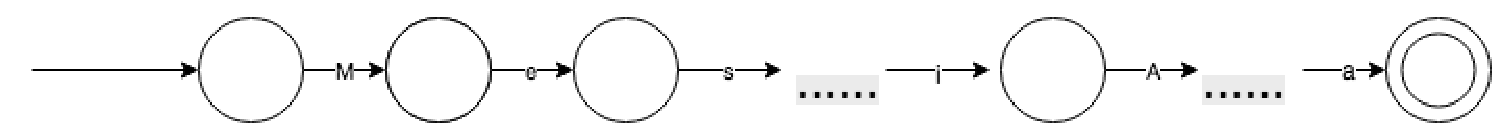
\includegraphics[scale=0.4]{lect3_img1.eps}
\end{unnumfigure}

$M_3$ accepts $L_1 \circ L_2$ $\Rightarrow$ $L_1 \circ L_2$ is regular.

\begin{definition}
    A \emph{non-deterministic finite automaton} is a 5-tuple $M = (Q, \Sigma, \delta, q_0, F)$ s.t.

    \begin{itemize}
        \item $Q, \Sigma, q_0, F$ are the same
        \item $\delta: Q \times (\Sigma \cup \{\epsilon\}) \rightarrow 2^Q$
        \begin{itemize}
            \item $\delta (q, s)$ is a subset of $Q$
        \end{itemize}
    \end{itemize}
\end{definition}

For a set $S$, $2^S$ is called the \emph{power set} of $S$. It contains all subsets of $S$.

$2^{\set{a, b}} = \set{\emptyset, \set{a}, \set{b}, \set{a, b}}$

\begin{definition}
    The NFA $M$ accepts the string  $w = w_1w_2 \ldots$ if there exists a string $y = y_1y_2 \ldots y_m \in (\Sigma \cup \set{\epsilon})^*$  and a sequence $r0, r_1, \ldots r_m \in Q$ such that:

    \begin{itemize}
        \item $w = y_1 \circ y_2 \circ \cdots \circ y_m$
        \item $r_0 = q_0$
        \item $r_i \in \delta (r_{i-1}, y_i) \text{ for } i = 1, \cdots, m$
        \item $r_m \in F$
    \end{itemize}
\end{definition}

Input string: $w = 00$

$y = \epsilon 00$, $r = q_0q_1q_2q_1$

$\delta(q_0, \epsilon) = \set{q_1, q_3}$

\section*{Lecture 4: Converting NFA-DFA, Operations on regular languages}

Language accepted by DFAs = Language accepted by NFAs = Regular Languages

Important properties of Regular Languages i.e. \emph{closure} properties. These are much easier to prove using NFAs.

\begin{theorem}[1.25 and 1.45 in texts]
    If $A$ and $B$ are regular, so is $A \cup B$ $\{x: x \in A \text{ or } x \in B\}$.
\end{theorem}

\begin{proof}
    The slide shows there is an NFA that accepts $A \cup B$.

    By theorem 1.39, $A \cup B$ is a regular language.
\end{proof}

\begin{theorem}
    Let $A$ and $B$ be regular. Then so are:

    \begin{itemize}
        \item Concatenation: $A \circ B = \set{x \circ y: x \in A, y \in B}$
        \item Star: $A^* = \set{x_1 \circ x_2 \circ \cdots \circ x_k: \text{ each } x_i \in A \text{ and } k \geq 0}$
        \item Complement: $\Sigma^* \diagdown A = \set{x: x \notin A}$
    \end{itemize}

    \emph{Note}: $\Sigma$ is in $A*$ $\rightarrow$ start state must be an accepting state
\end{theorem}

\begin{proof}
    (Theorem 1.39 and 1.40)

    \emph{Main claim}: Let $M = (Q, \Sigma, \delta, q_0, F)$ be an NFA. Let $L$ ba a language accepted by $M$. We can construct a DFA $M' = (Q', \Sigma, \delta', q_0, F)$ that also accepts $L$ (so $M$ and $M'$ are equivalent).

    First we need to define $\epsilon$-closure. For any set $S \subseteq Q$, let \emph{$E(S)$} be the set of all states in $Q$ that can be reached by following any number of $\epsilon$-transitions.

    \emph{Back to proof}:

    \begin{itemize}
        \item The states $Q' = 2^Q$ $\set{S: S \subseteq Q}$
        \item Accepting state $F' = \set{S \subseteq Q: \text{ any state in $S$ is an accepting state }} = \set{S \subseteq Q: S \cap F \neq \emptyset }$
    \end{itemize}

    \emph{Start state}: $q_0' = E(\set{q_0})$

    \emph{Transition function $\delta'$}:

    If NFA could be in states $S$, next input symbol is a, what states could it be in next?
    \begin{itemize}
        \item First, it could follow any $\epsilon$-transition, so could move to any state in $E(S)$.
        \item Next, unite $E(S) = \set{S_1, \ldots, S_n}$ could move to any state in $\delta(S_1, a) \cup \delta(S_2, a) \cup \ldots = \cup_{S \in E(S)} \delta(S, a)$.
        \item Again, it can follow any $\epsilon$-transitions
    \end{itemize}

    Final definition: $\delta'(S, a) = E(\cup_{S \in E(S)} \delta(S, a))$.
\end{proof}

\section*{Lecture 5: Regular expressions, Non-regular languages}

We will ``show'': A language is a regular iff it can be described by a \emph{regular expression}.

$R$:

\begin{itemize}
    \item $0^*1^*$
    \item $\Sigma^*001\Sigma^*$
    \item $(\Sigma\Sigma)^*$
    \item $\Sigma^*1\Sigma^*1\Sigma^*$
\end{itemize}

\emph{Shorthand}: $\Sigma = (a_1|a_2|\ldots|a_k) \text{ where } \Sigma  = a_1a_2\ldots a_k$

$L(R)$: the set of strings generated by regular expression $R$.

\begin{itemize}
  \item $\set{0^i1^j: i, j \geq 0}$
  \item \{all strings containing $001$ as a substring\}
  \item \{all strings of even length\}
  \item $\set{w: w \text{ contains at least three 1s}}$
\end{itemize}

$\Leftarrow$: Any regular expression can be converted into an equivalent NFA.

$\Rightarrow$: Idea: generalize NFAs by allowing arbitrary R.Es as labels on their transitions. Keep simplifying.

\emph{Limits to the power of Finite Automata}

Can any language be described by a F.A?

\begin{example}
    Suppose $L$ is a finite language (i.e. $L$ is finite). Is $L$ regular? Yes

    Why? Suppose $L = \set{x_1, \ldots, x_n}$.

    We can define $L_i = \set{x_i}$. This is regular. We know $L_1 \cup L_2$ is regular, so $L_1 \cup L_2 \cup \ldots \cup L_n$ is regular.

    This fails if $L$ is infinite because we could get an ``Infinite Automaton''.
\end{example}

\begin{example}
    Suppose $L$ is regular. Define $L^2 = \set{xy: x \in L \text{ and } y \in L}$

    This is regular: it is $L \circ L$.
\end{example}

\begin{example}
    $L^{dup} = \set{xx: x \in L}$

    Is this regular? It depends $\ldots$

    If $L$ is finite, $L^{dup}$ is finite, hence regular.

    If $L = L(1^*)$, then $L^{dup} = \set{1^{2i}: i \geq 0} = L((11)^*)$

    If $L = \Sigma^*$, $L^{dup} = \set{xx: x \in \Sigma^*}$. Is this regular?

    \emph{Intuitive argument}: $\set{xx: x \in \Sigma^*}$ is not regular.

    \begin{itemize}
        \item With a F.A. its states are its ``memory''.
        \item Any F.A. accepting $L^{dup}$ ``must remember'' the first half to compare to the second half.
        \item So F.A. must remember arbitrary large information, but it can't.
    \end{itemize}
\end{example}

\emph{Idea about finite automaton}:

\begin{unnumfigure}
    \includegraphics[scale=0.25]{lect5_img1}
\end{unnumfigure}

\begin{itemize}
    \item $\rightarrow$ ``computation path'', transitions followed when processing input
\end{itemize}

If input is very long, this computation path must have a \emph{cycle}.

\section*{Lecture 6: Pumping lemma: Proving languages are not regular}

$L = \set{w: w \text{ has a equal \# of occurrences of substrings 01 and 10 }}$

This \emph{is} a regular, surprisingly (Ex 1.48).

\begin{unnumfigure}
    \includegraphics[scale=0.2]{lect6_img1}
\end{unnumfigure}

Give the DFA a long input string $w$. \emph{Computation path on input $w$} must contain a cycle. Let $x$ be the part of input that was processed before arriving at $q$. While going round cycle, read $y$ from input. After cycle, we read $z$ from input.

What if input were $xyyz$. The DFA also accepts; we just travel cycle twice.

\emph{Message}: If $L$ is regular, then for a sufficiently long string $w \in L$, we can repeat its special substring $y$, to get another string in $L$.

\emph{Refinement of Message}: Let $p$ = \# states of DFA. If $|w| \geq p$ then computation path has length $\geq p + 1$. By Pigeonhole Principle, a cycle exists. So we can assume $\abs{xy} \leq p$. That's enough to get a cycle.

\emph{Important Point}:

\begin{itemize}
  \item We can (usually) use Pumping Lemma to prove that a language is not regular by proving that it satisfies the negation of Pumping Condition.
  \item We \emph{cannot} use P.L to prove that a language is regular.
\end{itemize}

How to negate a statement with logical quantifiers:

\begin{itemize}
  \item $\exists x$ s.t. $f$ becomes $\forall x$, NOT $f$
  \item $\forall x$, $g$ becomes $\exists x$ s.t. NOT $g$
\end{itemize}

\backmatter

\chapter{Context-Free Languages}

\section*{Lecture 7: Push down automata}

\begin{itemize}
    \item Only read input once, left to input
    \item Only finite memory
\end{itemize}

Basically, NFA with infinite stack (DFA + stack).

It turns out:
\begin{itemize}
    \item NFA + queue $\equiv$ Turing Machine
    \item NFA + 2 stacks $\equiv$ Turing Machine
\end{itemize}

Transitions of NFA now become: If in state $q$ and see symbol $a$ (or $\epsilon$) in input, and see $\sigma$ on stop of stack (or ignore it) then pop it, push $c$ onto the stack (or $\epsilon$) goto state $q'$ (if no transition $\rightarrow$ implicit reject).

\begin{example}[2.14 in text]
    $L = \{0^n1^n: n \geq 0\}$ This is not regular.
\end{example}

Exercise: $L = \{a^i b^j c^k: i, j, k \geq 0 and i = j \text{ or } i = k\}$

Hints:

\begin{enumerate}
  \item Need nondeterminism
  \item $L$ contains both $aabccc$ $(i = k)$ and $aabbc$ $(i = j)$
\end{enumerate}

\chapter{The Church-Turing Thesis}

\section*{Lecture 13: Examples of Multitape and Nondeterministic TMs}

\begin{example}
    $L = \{x\#x : x \in \Sigma^*\}$

    Let's do an implementation-level description of a multi-tape TM for $L$. Our original TM took time $\Theta(n^2)$ for inputs of length $n$.

    \begin{enumerate}
        \item Scan head 1 to the right until it reads a \#. Move Right. (Second head is still at start of tape 2)
        \item Repeatedly read symbol from tape 1, write it to tape 2, move both heads right, until seeing a blank on tape 1. Now second half of input is on tape 2.
        \item Move both heads left until they reach start of tapes (possibly using \$ back to find start of tape). Replace \# by $\textvisiblespace$ while doing so.
        \item Repeat until $\textvisiblespace$ on both tapes. If symbols differ, reject. Else, move both heads right.
    \end{enumerate}

    The multi-tape TM runs in $\Theta(n)$ time!
\end{example}

Last time: Configuration of TM, $aqb$, $a, b \in \Gamma^*$, $q \in Q$

Acceptance of a NTM: Input string is accepted if $\exists$ configurations $c_0, c_1, \ldots, c_k$ where:

\begin{itemize}
    \item $c_0 = q_{start} \; w$
    \item $c_i \Rightarrow c_{i+1}$ ($c_{i+1}$ is a possible configuration from $c_i$ following the transition function $\delta$)
    \item $c_k$ is on the accepting state
\end{itemize}

i.e. in a tree of configs, is there an accepting state:

\begin{enumerate}
    \item $w$ is accepted: any node in tree is an accepting state
    \item $w$ is explicitly rejected: the tree is finite, but yet no node is accepting config i.e. all leaves are rejection configs
    \item The NTM runs forever on $w$: the tree is infinite, but no node is accepting config
\end{enumerate}

\begin{definition}
    A NTM is a decider if for all inputs, case 1 or 2 happens.
\end{definition}

Example of NTMs: Let $L_1$, $L_2$ be recognizable languages. Let $M_i$ be a TM that recognizes $L_i$.

\emph{Claim}: $L_1 \cup L_2$ is recognizable. A cheat! Let's use nondeterminism.

\begin{definition}
    Define a NTM $M$ as follows:

    \begin{itemize}
        \item Nondeterministically choose to do one of the following:
        \begin{itemize}
            \item Run $M_1$
            \item Run $M_2$
        \end{itemize}
      \end{itemize}
\end{definition}

\emph{Claim}: $M$ recognizes $L_1 \cup L_2$.

\begin{proof}
    Suppose $w \in L_1 \cup L_2$. Say $w \in L_2$. Then the branch of tree simulating $M_i$ will accept. So $M$ is in case 1, and accepts. If $w \notin L_1 \cup L_2$, then both $M_1 \& M_2$ either run forever or reject. So $M$ is in either case 2 and case 3. So $M$ does not accept $w$.
\end{proof}

\begin{theorem}
    Given a NTM $M$, we can construct a DTM $M$ s.t. $L(M) = L(M')$.
\end{theorem}

\begin{theorem}
    If $M$ is a NTM decider, then we can make $M'$ a decider as well.
\end{theorem}

Using Theorem, we get a DTM $M'$, completing proof of claim 1.

\backmatter
% \appendix
\chapter{This is Appendix Title}

\section{This is First Level Heading}
\lipsum[1-2]

\subsection{This is Second Level Heading}
\lipsum[3]

\subsubsection{This is Third Level Heading}
\lipsum[4]

\paragraph{This is Fourth Level Heading}
\lipsum[5]

\subparagraph{This is Fifth Level Heading}
\lipsum[6]

%\backmatter

%\bibliography{wiley}%



\latexprintindex

\end{document}
